\documentclass
[
  draft    = true,
  fontsize = 11pt,
  parskip  = half-,
  BCOR     = 0pt,
  DIV      = 11,
  ngerman,
  dvipsnames
]
{scrartcl}

% Standardpakete
\usepackage{fixltx2e}
\usepackage[utf8]{inputenc}
\usepackage[T1]{fontenc}
\usepackage{lmodern}
\usepackage{babel}
% Zusatzpakete
\usepackage{amsmath}
\usepackage{amssymb}
\usepackage{tikz}


% ------------------------------------------------------------------------------
\begin{document}
% ------------------------------------------------------------------------------

% --------------------------------------
\section*{Transformation von Funktionen}
%---------------------------------------
Translation:
\begin{alignat*}{2}
  g(x)&=f(x)+a      & \quad&\text{bewirkt eine Verschiebung in $y$-Richtung} \\
  g(x)&=f(x+a)      & \quad&\text{bewirkt eine Verschiebung in $x$-Richtung}
\intertext{Skalierung:}
  g(x)&=a\cdot f(x) & \quad&\text{bewirkt eine Streckung bzw. Stauchung in $y$-Richtung} \\
  g(x)&=f(a\cdot x) & \quad&\text{bewirkt eine Streckung bzw. Stauchung in $x$-Richtung}
\intertext{Reflexion (Spezialfall einer Skalierung):}
  g(x)&=-f(x)       & \quad&\text{$a=-1$ bewirkt hier eine Spiegelung an der $x$-Achse}  \\
  g(x)&=f(-x)       & \quad&\text{$a=-1$ bewirkt hier eine Spiegelung an der $y$-Achse}
\end{alignat*}

Der Einfluss von $a$:
\begin{center}
  % vertikale Mindesthoehe
  \newcommand{\vstrut}{\rule[-0.7ex]{0pt}{2.7ex}}%
  % Translation
  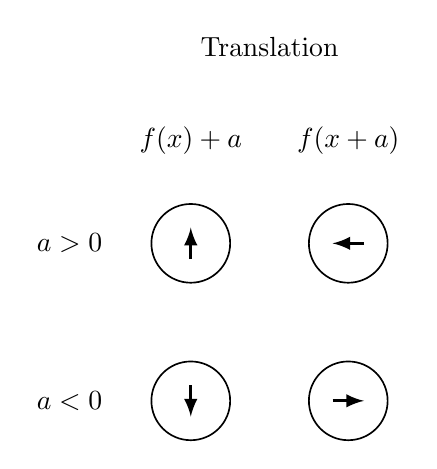
\begin{tikzpicture}
    % Terme
    \node        at ( 1, 4.5) {\vstrut Translation};
    \node[above] at ( 0, 3.0) {\vstrut$f(x)+a$};
    \node[above] at ( 2, 3.0) {\vstrut$f(x+a)$};
    \node[left]  at (-1, 2.0) {\vstrut$a>0$};
    \node[left]  at (-1, 0.0) {\vstrut$a<0$};
    % Verschiebung nach oben (oben links)
    \begin{scope}[xshift=0cm, yshift=2cm]
      \draw[line width=0.6pt] (0, 0) circle[radius=5mm];
      \draw[line width=1.2pt, ->, >=latex] (0, -2mm) -- (0, 2mm);
    \end{scope}
    % Verschiebung nach links (oben rechts)
    \begin{scope}[xshift=2cm, yshift=2cm]
      \draw[line width=0.6pt] (0, 0) circle[radius=5mm];
      \draw[line width=1.2pt, ->, >=latex] (2mm, 0) -- (-2mm, 0);
    \end{scope}
    % Verschiebung nach unten (unten links)
    \begin{scope}[xshift=0cm, yshift=0cm]
      \draw[line width=0.6pt] (0, 0) circle[radius=5mm];
      \draw[line width=1.2pt, ->, >=latex] (0, 2mm) -- (0, -2mm);
    \end{scope}
    % Verschiebung nach rechts (unten rechts)
    \begin{scope}[xshift=2cm, yshift=0cm]
      \draw[line width=0.6pt] (0, 0) circle[radius=5mm];
      \draw[line width=1.2pt, ->, >=latex] (-2mm, 0) -- (2mm, 0);
    \end{scope}
  \end{tikzpicture}
  \hspace{2cm}
  % Skalierung
  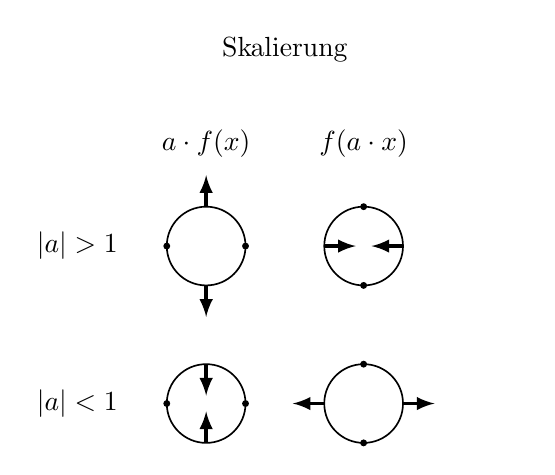
\begin{tikzpicture}
    % Terme
    \node        at ( 1, 4.5) {\vstrut Skalierung};
    \node[above] at ( 0, 3.0) {\vstrut$a\cdot f(x)$};
    \node[above] at ( 2, 3.0) {\vstrut$f(a\cdot x)$};
    \node[left]  at (-1, 2.0) {\vstrut$\vert a\vert>1$};
    \node[left]  at (-1, 0.0) {\vstrut$\vert a\vert<1$};
    \node[right] at ( 3, 2.0) {\hphantom{\vstrut$a>0$}};
    \node[right] at ( 3, 0.0) {\hphantom{\vstrut$a<0$}};
    % Streckung in y-Richtung (oben links)
    \begin{scope}[xshift=0cm, yshift=2cm]
      \draw[line width=0.6pt] (0, 0) circle[radius=5mm];
      \draw[line width=1.2pt, ->, >=latex] (0,  5mm) -- (0,  9mm);
      \draw[line width=1.2pt, ->, >=latex] (0, -5mm) -- (0, -9mm);
      \fill (-5mm, 0) circle[radius=1.25pt];
      \fill ( 5mm, 0) circle[radius=1.25pt];
    \end{scope}
    % Stauchung in x-Richtung (oben rechts)
    \begin{scope}[xshift=2cm, yshift=2cm]
      \draw[line width=0.6pt] (0, 0) circle[radius=5mm];
      \draw[line width=1.2pt, ->, >=latex] (-5mm, 0) -- (-1mm, 0);
      \draw[line width=1.2pt, ->, >=latex] ( 5mm, 0) -- ( 1mm, 0);
      \fill (0, -5mm) circle[radius=1.25pt];
      \fill (0,  5mm) circle[radius=1.25pt];
    \end{scope}
    % Stauchung in y-Richtung (unten links)
    \begin{scope}[xshift=0cm, yshift=0cm]
      \draw[line width=0.6pt] (0, 0) circle[radius=5mm];
      \draw[line width=1.2pt, ->, >=latex] (0,  5mm) -- (0,  1mm);
      \draw[line width=1.2pt, ->, >=latex] (0, -5mm) -- (0, -1mm);
      \fill (-5mm, 0) circle[radius=1.25pt];
      \fill ( 5mm, 0) circle[radius=1.25pt];
    \end{scope}
    % Streckung in x-Richtung (unten rechts)
    \begin{scope}[xshift=2cm, yshift=0cm]
      \draw[line width=0.6pt] (0, 0) circle[radius=5mm];
      \draw[line width=1.2pt, ->, >=latex] (-5mm, 0) -- (-9mm, 0);
      \draw[line width=1.2pt, ->, >=latex] ( 5mm, 0) -- ( 9mm, 0);
      \fill (0, -5mm) circle[radius=1.25pt];
      \fill (0,  5mm) circle[radius=1.25pt];
    \end{scope}
  \end{tikzpicture}
\end{center}

\clearpage
Beispiel:\quad $f(x)=x^{3}-3x^{2}-x+3$\par
\begin{center}
  \begin{tikzpicture}[scale=0.5]
    \begin{scope}[yshift=7cm]
      \begin{scope}[xshift=-7cm]
        % Transformationsforschrift (Verschiebung in y-Richtung)
        \node[below right] at (-6, 6) {{\small$g(x)=f(x)+a$}};
        % Koordinatenachsen
        \draw[line width=0.8pt, ->, >=latex] (-6, 0) -- (6, 0) node[below left] {{\small$x$}};
        \draw[line width=0.8pt, ->, >=latex] (0, -6) -- (0, 6);
        % Funktionen
        \begin{scope}
          \clip (-6, -6) rectangle (6, 6);
          \draw[line width=0.6pt, draw=red]   plot[smooth] file{octave/transy-pos.xy};
          \draw[line width=0.6pt, draw=blue]  plot[smooth] file{octave/transy-neg.xy};
          \draw[line width=0.6pt, draw=black] plot[smooth] file{octave/f.xy};
        \end{scope}
        % Summanden
        \node[left]              at (-1.9, -5.6) {{\small\textcolor{red}{$a=2$}}};
        \node[right, fill=white] at (-1.3, -5.6) {{\small\textcolor{blue}{$a=-2$}}};
      \end{scope}
      \begin{scope}[xshift=7cm]
        % Transformationsforschrift (Verschiebung in x-Richtung)
        \node[below right] at (-6, 6) {{\small$g(x)=f(x+a)$}};
        % Koordinatenachsen
        \draw[line width=0.8pt, ->, >=latex] (-6, 0) -- (6, 0) node[below left] {{\small$x$}};
        \draw[line width=0.8pt, ->, >=latex] (0, -6) -- (0, 6);
        % Funktionen
        \begin{scope}
          \clip (-6, -6) rectangle (6, 6);
          \draw[line width=0.6pt, draw=blue]  plot[smooth] file{octave/transx-pos.xy};
          \draw[line width=0.6pt, draw=red]   plot[smooth] file{octave/transx-neg.xy};
          \draw[line width=0.6pt, draw=black] plot[smooth] file{octave/f.xy};
        \end{scope}
        % Faktoren
        \node[right] at ( 0.0, -5.6) {{\small\textcolor{red}{$a=-1,\!5$}}};
        \node[left]  at (-3.0, -5.6) {{\small\textcolor{blue}{$a=1,\!5$}}};
      \end{scope}
    \end{scope}
    \begin{scope}[yshift=-7cm]
      \begin{scope}[xshift=-7cm]
        % Transformationsforschrift (Skalierung in y-Richtung)
        \node[below right] at (-6, 6) {{\small$g(x)=a\cdot f(x)$}};
        % Koordinatenachsen
        \draw[line width=0.8pt, ->, >=latex] (-6, 0) -- (6, 0) node[below left] {{\small$x$}};
        \draw[line width=0.8pt, ->, >=latex] (0, -6) -- (0, 6);
        % Funktionen
        \begin{scope}
          \clip (-6, -6) rectangle (6, 6);
          \draw[line width=0.6pt, draw=red]   plot[smooth] file{octave/scaley-big.xy};
          \draw[line width=0.6pt, draw=blue]  plot[smooth] file{octave/scaley-sml.xy};
          \draw[line width=0.6pt, draw=black] plot[smooth] file{octave/f.xy};
        \end{scope}
        % Faktoren
        \node[right, fill=white] at (-1.3, -5.6) {{\small\textcolor{red}{$a=1,\!8$}}};
        \node[left]              at (-2.5, -5.6) {{\small\textcolor{blue}{$a=0,\!2$}}};
      \end{scope}
      \begin{scope}[xshift=7cm]
        % Transformationsforschrift (Skalierung in x-Richtung)
        \node[below right] at (-6, 6) {{\small$g(x)=f(a\cdot x)$}};
        % Koordinatenachsen
        \draw[line width=0.8pt, ->, >=latex] (-6, 0) -- (6, 0) node[below left] {{\small$x$}};
        \draw[line width=0.8pt, ->, >=latex] (0, -6) -- (0, 6);
        % Funktionen
        \begin{scope}
          \clip (-6, -6) rectangle (6, 6);
          \draw[line width=0.6pt, draw=blue]  plot[smooth] file{octave/scalex-big.xy};
          \draw[line width=0.6pt, draw=red]   plot[smooth] file{octave/scalex-sml.xy};
          \draw[line width=0.6pt, draw=black] plot[smooth] file{octave/f.xy};
        \end{scope}
        % Faktoren
        \node[left]              at (-2.5, -5.6) {{\small\textcolor{red}{$a=0,\!6$}}};
        \node[right, fill=white] at (-0.7, -5.6) {{\small\textcolor{blue}{$a=1,\!8$}}};
      \end{scope}
    \end{scope}
  \end{tikzpicture}
\end{center}

\begin{center}
  \begin{tikzpicture}[scale=0.5]
    \begin{scope}[xshift=-7cm]
      % Transformationsforschrift (Spiegelung an der x-Achse)
      \node[above right] at (-6, 6) {{\small$g(x)=-f(x)$}};
      % Koordinatenachsen
      \draw[line width=0.8pt, ->, >=latex] (-6, 0) -- (6, 0) node[below left] {{\small$x$}};
      \draw[line width=0.8pt, ->, >=latex] (0, -6) -- (0, 6);
      % Funktionen
      \begin{scope}
        \clip (-6, -6) rectangle (6, 6);
        \draw[line width=0.6pt, draw=blue]  plot[smooth] file{octave/reflectx.xy};
        \draw[line width=0.6pt, draw=black] plot[smooth] file{octave/f.xy};
      \end{scope}   
    \end{scope}
    \begin{scope}[xshift=7cm]
      % Transformationsforschrift (Spiegelung an der y-Achse)
      \node[above right] at (-6, 6) {{\small$g(x)=f(-x)$}};
      % Koordinatenachsen
      \draw[line width=0.8pt, ->, >=latex] (-6, 0) -- (6, 0) node[below left] {{\small$x$}};
      \draw[line width=0.8pt, ->, >=latex] (0, -6) -- (0, 6);
      % Funktionen
      \begin{scope}
        \clip (-6, -6) rectangle (6, 6);
        \draw[line width=0.6pt, draw=blue]  plot[smooth] file{octave/reflecty.xy};
        \draw[line width=0.6pt, draw=black] plot[smooth] file{octave/f.xy};
      \end{scope}   
    \end{scope}
  \end{tikzpicture}
\end{center}

% ------------------------------------------------------------------------------
\end{document}
% ------------------------------------------------------------------------------

